\documentclass[../bericht.tex]{subfiles}

\begin{document}

  \chapter{The Experiment}

    \section{Experimental setup and conduction}
    \label{sec:exp-setup}

      \begin{figure}[bt]
        \centering
        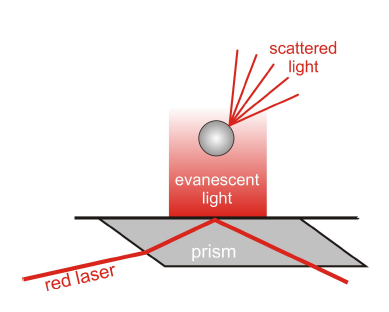
\includegraphics[width=0.5\textwidth]{figures/eyp_setup.png}
        \caption{Relevant part of the experimental setup. The light of the evanescent field is scattered by the colloidal particles. For more explanations, please refer to \cref{sec:exp-setup}.}
        \label{fig:exp-setup}
      \end{figure}

      The experimental setup focuses on a glass cuvette holding an aqueous dispersion with colloidal particles. \Cref{fig:exp-setup} shows the relevant part of the experimental setup. Through a prism, a red laser beam is focused on the sample at such an angle, that the beam is totally reflected and only an evanescent light field reaches the colloidal particles. This light is scattered and it's intensity measured at a fixed angle. Simultaneously, a green laser beam is used as an optical tweezer to hold the single particle in place which the red laser is focused on. Depending on the power of the green laser, the particle is trapped in a trap of varying strength.
      \medskip

      Using the optical tweezers, a single colloidal particle is trapped. It can be tracked using the footage of a camera. Once the particle is centered on the computer screen by moving the sample holder in a plane not affecting the angles of the incident laser beams, a different objective is rotated in front of the camera, resulting in a stronger amplification. Again, the particle is centered on the computer screen. Then, the intensity of the scattered light is recorded by a computer program over the duration of $\SI{20}{\minute}$. Here, it is important to check from time to time, that the particle has not escaped from the optical tweezers.

      This process is repeated for different input voltages of the optical tweezers' green laser: $U_\mathrm{tweezers}=\SI{0,76}{\volt},\SI{0,70}{\volt},\SI{0,65}{\volt},\SI{0,60}{\volt},\SI{0,00}{\volt}$. To measure the spectrum with the optical tweezers turned off, a particle is focused on analogously to the process with the optical tweezers turned on. During the measurement, the position of the sample holder must continuously be readjusted to track the particle.

      Then, a spectrum at $U_\mathrm{tweezers}=\SI{0,75}{\volt}$ is recorded at a larger incident angle of the red laser (in respect to the normal of the prism's surface and the beam (compare \cref{fig:exp-setup})). Finally, a dark spectrum of the background noise is taken with the red laser turned off.

      \begin{figure}[tb]
        \centering
        \subfloat[]{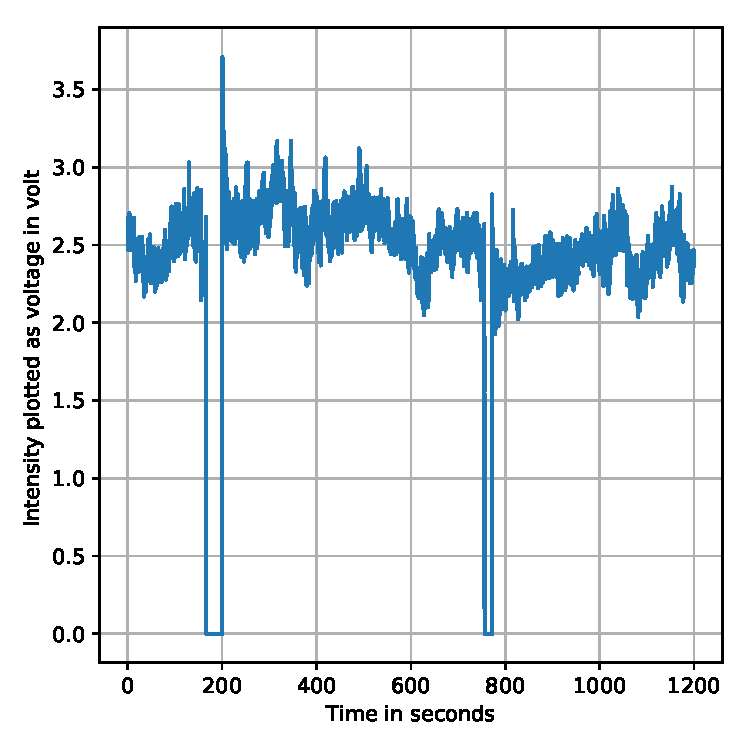
\includegraphics[width=0.45\textwidth]{figures/intensity_time.pdf} \label{fig:i-t-70}}
        \hfill
        \subfloat[]{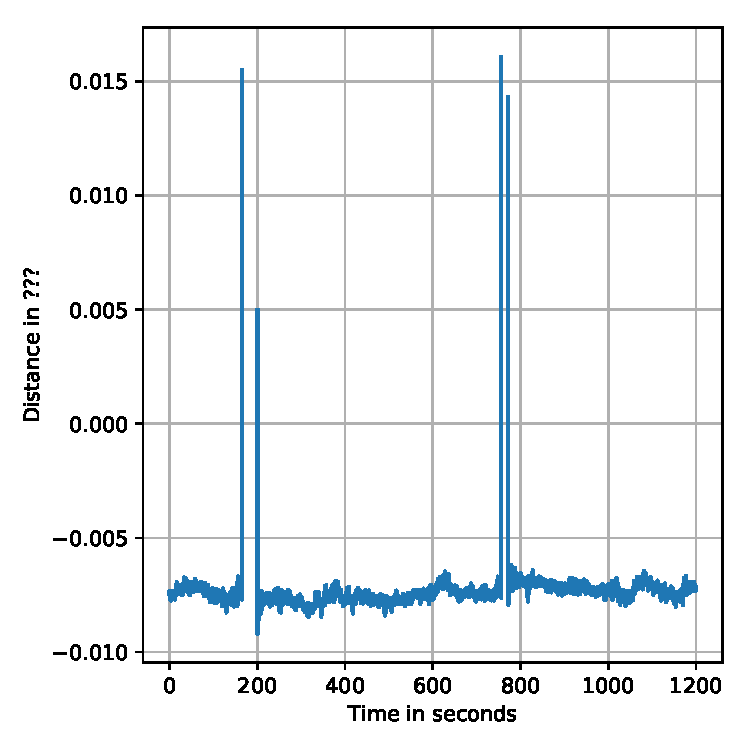
\includegraphics[width=0.45\textwidth]{figures/distance_time.pdf} \label{fig:z-t-70}}
        \caption{Plots of the recorded raw data with the optical tweezers voltage $U_\mathrm{tweezers}=\SI{0,70}{\volt}$. \protect\subref{fig:i-t-70} Recorded raw data: Intensity of the scattered light over time. \protect\subref{fig:i-t-70} Same data with a processed intensity axis, now showing the distance $z$ between particle and cuvettes walls ($I_0^{70}=2,6$).}
        \label{fig:70-i-t-z-t}
      \end{figure}


    \section{Data analysis}
    \label{sec:data-analysis}

       The $I_0$ values are determined by a trial and error method.
       We plotted:
       \begin{align*}
         I(z)&=I_0 \exp\left( -\beta z \right)
       \end{align*}
       for different $I_0$ values and compared it to our measured I(z) date as seen in \cref{eq:I0determination}.

        \begin{figure}[tb]
              \centering
              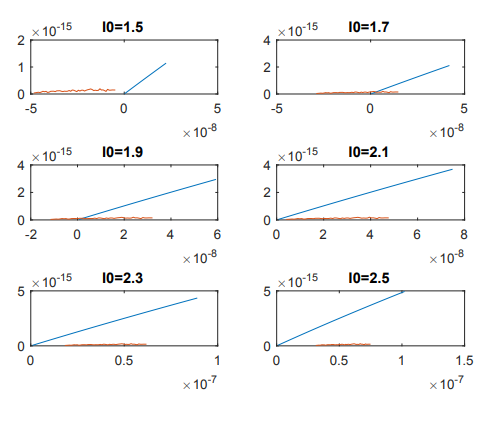
\includegraphics[width=0.70\textwidth]{figures/I0determination.PNG}
              \caption{Plotted and measured intensity curves layered to find the best fit for $I_0$. The red line is the measured data, the blue line is the plot and $I_0= 1,9$ was chosen as the best fit. }
              \label{fig:I0determination}
        \end{figure}

        The $I_0$ value were both plots are the closest to each other is chosen. With this set of diagrams we determined the $I_0$ value for the $U_\mathrm{tweezers}=\SI{0,75}{\volt}$ data-set. This was the best looking data-set for $I_0$ determination,but to not cause any confusion, the measurements conducted for $U_\mathrm{tweezers}=\SI{0,75}{\volt}$ did not yield any usable results. There are a lot of \textit{nan} values in the data set, which could therefore not be processed as the other sets. This might be due to the particle being lost from time to time. It is not really clear, as the particle has been observed most of the time of the measurement.
        \medskip

      In the following, the step by step evaluation is written down for a new exemplary measurement data set, but $I_0$ is determined by the same process. To this end, the measurement with the optical tweezers voltage $U=\SI{0,70}{\volt}$ is analyzed in detail.  The other measurements are analyzed analogously and therefore,only the results will be presented for each step.
      \medskip

      \begin{figure}[tb]
        \centering
        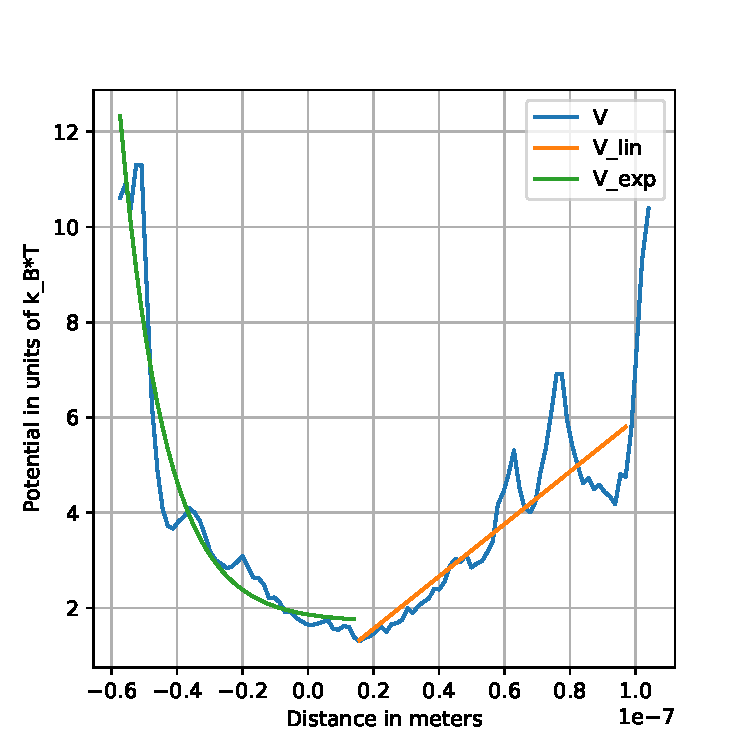
\includegraphics[width=0.45\textwidth]{figures/70_potential.pdf}
        \caption[Potential computed for the tweezers voltage $U_\mathrm{tweezers}=\SI{0,70}{\volt}$.]{Potential computed for the tweezers voltage $U_\mathrm{tweezers}=\SI{0,70}{\volt}$. The potential is divided in two overlaying sub-potentials and the respecting fits (compare \cref{eq:pot-fits}) plotted on top of the potential.}
        \label{fig:potential-with-fits-70}
      \end{figure}

      \Cref{fig:i-t-70} shows the recorded raw data: The intensity of the scattered light $I(z)$ over a time axis. As the measurement of the background noise yielded a constant zero signal, the correction is irrelevant.  $z$ is the distance between the colloidal particle at the wall of the cuvette. The dependency of $I$ on $z$ is given by
      \begin{align}
        I(z)&=I_0 \exp\left( -\beta z \right)  \\
        \Rightarrow \quad z&=-\beta^{-1} \ln \left(\frac{I(z)}{I_0}\right)=-\beta^{-1}\ln I(z) + \beta^{-1}\ln I_0,
      \end{align}
      where $\beta^{-1}$ is the penetration depth of the evanescent field and $I_0$ the scatter intensity that results when particles and wall are in direct contact. At this point, only relative distances can be computed as $I_0$ is an unknown constant. As this constant will be computed in the course of this evaluation, the graph shown in \cref{fig:z-t-70} uses the absolute distance data with the parameter $I_0^{70}=2,6$. With \cref{eq:potential} in combination with the determined  $I_0^{70}=2,6$ the potential can be calculated.

      \medskip

      The computed potential $V(z)$ of the measurements is illustrated in \cref{fig:potential-with-fits-70} Using the potential's minimum as a breakpoint, it can be divided into two overlaying potentials: An exponential potential for the sharp drop at the beginning, and a linear rising after the minimum signifying the gravitational and the light force. The so divided sections of the potential are fitted with an exponential and a linear curve:
      \begin{align}
        \begin{split}
          V_\mathrm{exp}(z) &= a\cdot \exp\left( -b z \right) + c \\
          V_\mathrm{lin}(z) &= mz+ d.
        \end{split}
        \label{eq:pot-fits}
      \end{align}
      A small data modification needs to be done yet: The potential data is derived from a histogram that sorts by intervals of the Boltzmann distribution. Therefore, the potential data points at high distance values contain only few scattered photons and can therefore be neglected. All in all, the selection of the interval to be fitted with a linear fit is more or less an approximation o the authors to reach the wanted results. These results are plotted in \cref{fig:potential-with-fits-70} along with the potential itself.

      At this point, the data of $I_\mathrm{tweezers}=\SI{0}{\volt}$ is used, to determine the gravitational potential. Because in the respective potential, there is no light force to be had since the laser has been turned off during the experiment, the linear part manifests only due to the gravitational potential. Taking the gradient of this potential, which is simply the slope of the fit in this case, the gravitation force on the particle is derived to be
      \begin{equation*}
        F_\mathrm{gravitational}^\mathrm{experimental}\approx\SI{3,9e-13}{\newton}\approx \SI{4,0e-13}{\newton}=\frac{4}{3}\pi r_\mathrm{particle}^3= \rho_\mathrm{Polysterene}*g=F_\mathrm{gravitational}^\mathrm{theoretical},
      \end{equation*}
      where $g=\SI{9,81}{\meter\per\square\second}$ is the gravitational acceleration on earth's surface, $r_\mathrm{particle}=\frac{a}{2}=\SI{2,14e-6}{\meter}$ the particle's radius and $\rho_\mathrm{Polysterene}$ the mass density of polysterene. Since the fit intervall has been optimized to hit close to the theoretical value, there is no way of approximating the uncertainties. The fit parameter error is only a very small secondary error. What could be done for a more precise evaluation is to weigh the different data points using the values of the histogram used to derive the potential form or even using the Boltzmann distribution as a weight.
      \medskip

      The light force of the other measurements is now determined by subtracting the linear fit of $I_\mathrm{tweezers}=\SI{0}{\volt}$ from the other linear fits, in explanation
      \begin{equation}
          V_\mathrm{Light-Force} = V_\mathrm{lin} - V_\mathrm{Gravitational},
          \label{eq:light-forces}
      \end{equation}
      with the light force potential $V_\mathrm{Light-Force}$, the total linear potential $V_\mathrm{lin}$ and the gravitational potential $V_\mathrm{gravitational}$. The results for all measurements are plotted in \cref{fig:light-forces}. Since increasing the voltage of the optical tweezers linearly scales with the number of emitted photons (the wavelength is constant), a linear scaling between light force and the tweezers' voltage is expected. The before mentioned figure shows exactly that, the light forces being
      \begin{align*}
        F_\mathrm{Light-Force}(U_\mathrm{tweezers}=\SI{0,70}{\volt})=\SI{-1,6e-13}{\newton} \\
        F_\mathrm{Light-Force}(U_\mathrm{tweezers}=\SI{0,65}{\volt})=\SI{-1,0e-13}{\newton} \\
        F_\mathrm{Light-Force}(U_\mathrm{tweezers}=\SI{0,60}{\volt})=\SI{-0,5e-13}{\newton} .
      \end{align*}
      As a result, expectations are that the linear part of the potentials becomes steeper for higher voltages of $U_\mathrm{tweezers}$. \Cref{fig:potentials} shows the comparison of all the measured potentials. As a matter of fact, the expectations are not satisfied by that comparison. The potentials' forms are seem to be disturbed too much to yield a clear tendency. Maybe bigger steps of $U_\mathrm{tweezers}$ would yield a more suggestive image.
      \medskip

      \begin{figure}[tb]
        \centering
        \subfloat[]{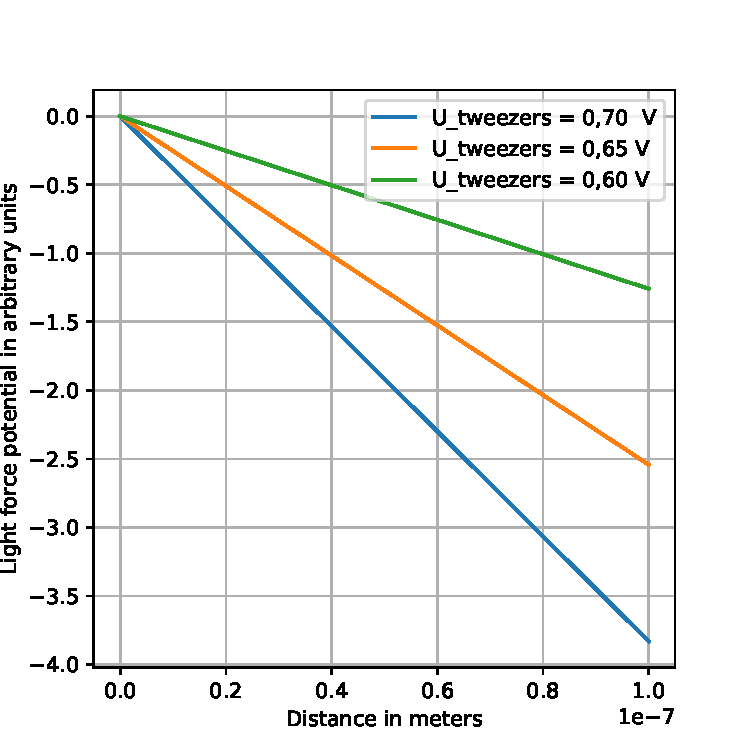
\includegraphics[width=0.45\textwidth]{figures/light_forces.pdf} \label{fig:light-forces}}
        \hfill
        \subfloat[]{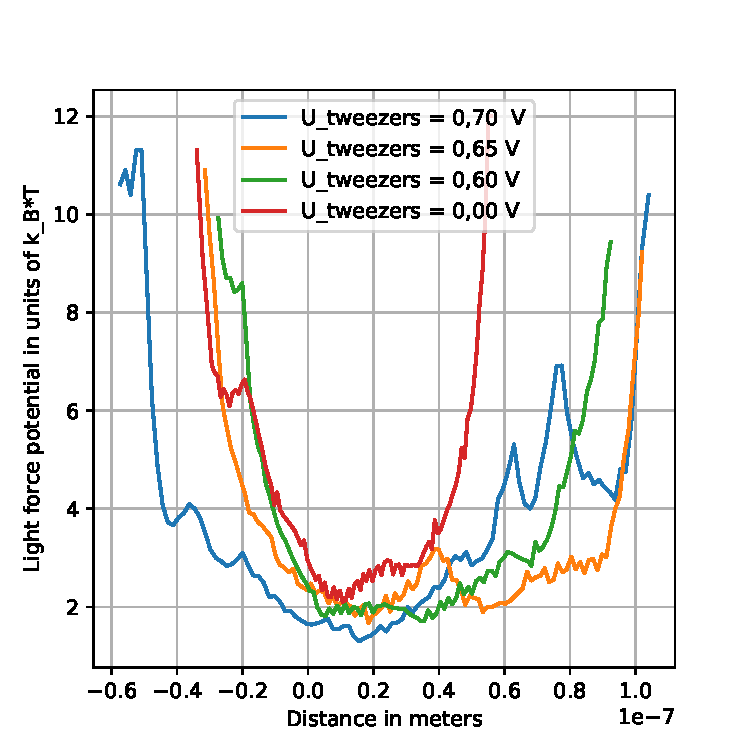
\includegraphics[width=0.45\textwidth]{figures/potentials.pdf} \label{fig:potentials}}
        \caption{\protect\subref{fig:light-forces} Computed light forces (compare \cref{eq:light-forces}) for the different voltages $U_\mathrm{tweezers}$ of the optical tweezers. \protect\subref{fig:potentials} Comparison of all the measured potentials.}
      \end{figure}

      Finally, \cref{fig:two-blocks} shows the influence of the penetration depth of the evanescent field. Both measurements have been conducted at approximately the same tweezers voltage $U_\mathrm{tweezers}=\SI{0,76}{\volt}\approx \SI{0,75}{\volt}$. The penetration depth has been varied by changing the incident angle of the red laser onto the prism. The only significant difference between the two potentials is the shift to higher distances for the smaller penetration depth.

      \begin{figure}[tbh]
        \centering
        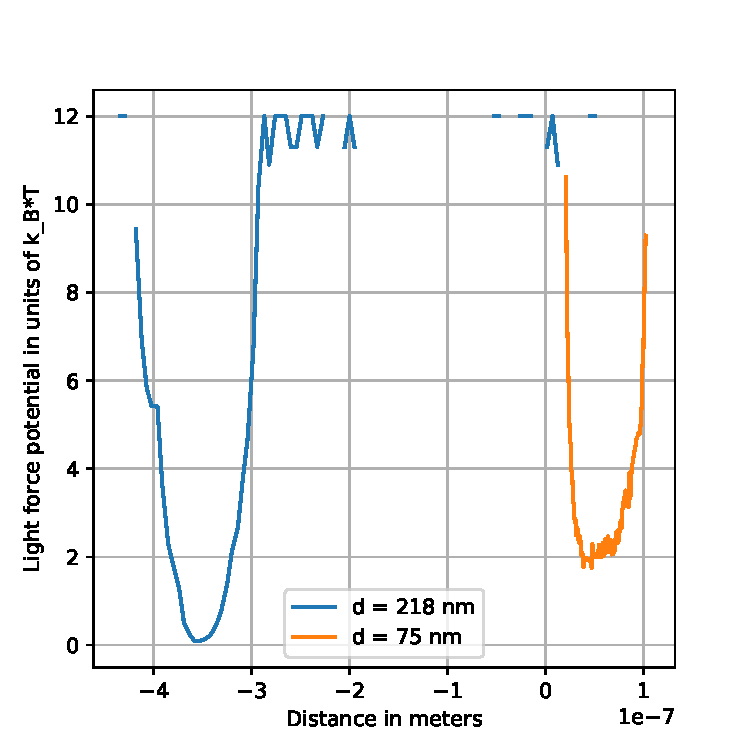
\includegraphics[width=0.45\textwidth]{figures/potentials12.pdf}
        \caption{Comparison of the potentials derived from two measurements when varying the penetration depth of the evanescent field.}
        \label{fig:two-blocks}
      \end{figure}







\end{document}
